%% chapter 1

\chapter{绪论}
  在病毒或细菌感染期间,免疫因子会在人体中释放,通常会导致组织发炎并导致严重的疾病行为,例如食欲不振,嗜睡,退出正常的社交活动,疲劳,探索力下降,嗜睡,运动性快感不足,并减少情绪。

  人们认为疾病行为是由可溶性促炎性细胞因子触发的,该因子由感染部位的免疫细胞产生。一些主要的促炎细胞因子包括interleukin-1(IL-1),tumor necrosis factor alpha$\alpha$(TNF-$\alpha$)和interleukin-6(IL-6)。如所报道的,这些源自免疫系统和免疫细胞的促炎细胞因子可对神经内分泌系统,特别是下丘脑-垂体-肾上腺(HPA)轴产生深远的影响。

  HPA轴是体内的压力反应中心,连接中枢神经系统(CNS)和内分泌系统。 HPA轴的激活导致下丘脑释放促肾上腺皮质激素释放激素(CRH),促使垂体释放肾上腺皮质激素(ACTH)和肾上腺糖皮质激素(人体内糖皮质激素的活性形式是皮质醇,而啮齿动物中的皮质激素是皮质甾酮)。糖皮质激素作用于下丘脑和垂体,对免疫细胞产生负反馈,以抑制细胞因子的进一步合成和释放(图\ref{fig:HPA}),从而保护宿主免受过度活跃的免疫反应的有害影响。

\begin{figure}[!htb]
  \centering
  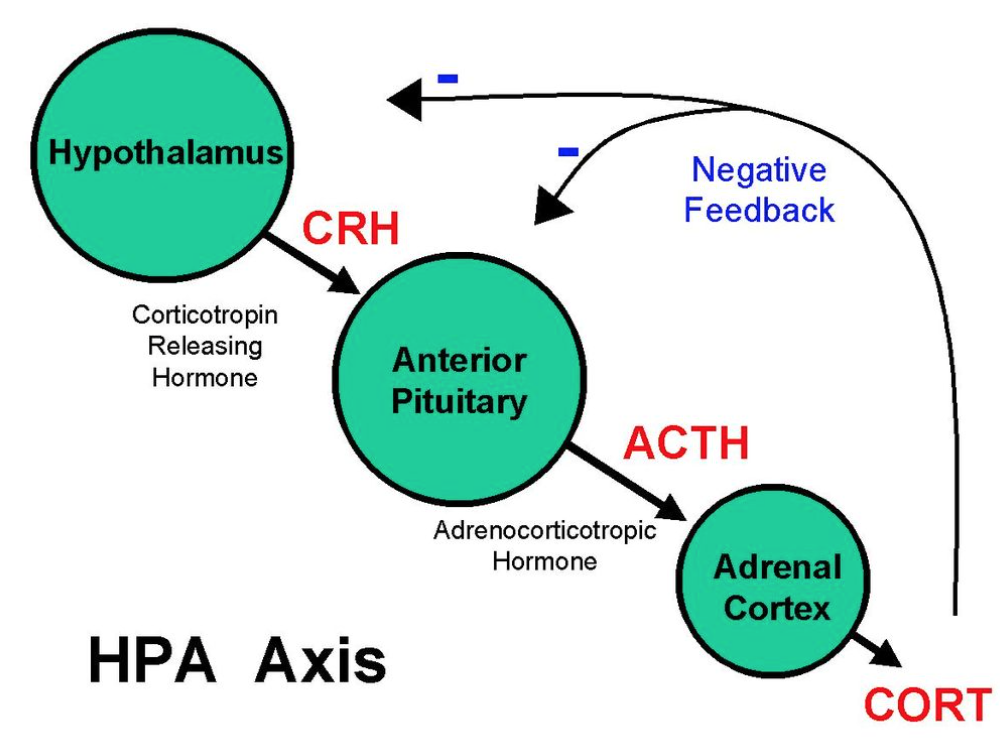
\includegraphics[width=0.6\textwidth]{figs/HPA.png}
  \caption{炎症状态下的HPA轴}
  \label{fig:HPA}
\end{figure}

  重要的是,由炎症事件诱导的细胞因子(IL1,IL6,TNF-$\alpha$,IFN-$\gamma$)通常循环至垂体前叶,并主要作用于垂体的促肾上腺皮质激素,从而促进释放抗炎激素,例如肾上腺皮质激素(ACTH)。 ACTH被携带到肾上腺并作用于ACTH受体,从而上调肾上腺皮质肾上腺皮质细胞中皮质醇的释放。随后,皮质醇在下丘脑和垂体在HPA轴上产生负反馈,以抑制促炎性细胞因子的进一步合成和释放。

  此外,卵泡细胞代表垂体前叶中唯一的非内分泌细胞类型,并释放可能潜在影响垂体局部激素产生的IL1和IL6,从而构成调节炎症反应的复杂系统。

  因此,垂体积极参与炎症事件的调节。我们推测,基于垂体细胞转录谱的分析,对垂体细胞进行彻底和详细的分类,可以为后续研究其在炎症事件中的功能提供有价值的资源。

  文章的主要贡献如下:
\begin{itemize}
    \item 建立了一个涉及多种免疫刺激剂、多尺度给药剂量与恢复时程的小鼠炎症模型,并在单细胞水平上提供了其垂体细胞测序数据。
    \item 揭示了不同种类垂体细胞在参与中枢神经内分泌炎症调节的过程中的转录水平差异,表明其在炎症调节过程中扮演不同的角色。
    \item 发现了一类在不同种类垂体细胞中统一表达的转录因子,表明其在垂体参与中枢神经内分泌炎症调节过程中的重要地位。
\end{itemize}

  文章结构安排如下:第二章介绍单细胞测序以及基因调控网络(GRN)的相关工作;第三章介绍SCENIC算法原理;第四章介绍实验设计,包括小鼠垂体单细胞测序、搭建小鼠炎症模型以及验证炎症条件下生物标志物;第五章介绍使用GRN对小鼠垂体单细胞测序数据进行分析;第六章总结了我们的结论。

